

Projektin viikkopalaverissa päätettiin, että sivut pitäisi pystyä kääntämään usealle kielelle.
Alkuperin ei ollut suunniteltu käännöksiä, joten kaikki teksti sivuilla oli kovakoodattu komponentteihin suomeksi. 
Tämä vaatisi paljon työtä kovakoodattujen sanojen ja lauseiden etsimistä koodipohjasta ja niitten vaihtoa johonkin muotoon, jossa teksti voidaan vaihtaa eri kielille.
\medskip

Tavoitteena oli kääntää sivut englanniksi, suomeksi ja saksaksi. Käännösjärjestelmän pitäisi myös olla laajennettava, jotta siihen voisi lisätä enemmän kieliä tulevaisuudessa.
Projektin teknisen johdon kanssa päätettiin käyttää Meteorin tukemaa i18n kirjastoa, joka on suunniteltu helposti laajennettavaksi.
\medskip







\subsection*{I18n}


Sana i18n tarkoittaa englannin sanaa "internationalization"{} (suom. kansainvälistyminen), jossa 18 tarkoittaa kirjainmäärää 'i' ja 'n' kirjainten välillä. Projektissa käytetään meteor-universe-i18n JavaScript kirjastoa, joka tuo monta käännösten tekemiseen tarvittua työkalua.
Kirjasto on suunniteltu alusta asti Meteorin käyttötarkoituksiin.\medskip

i18n käännösprosessi vaatii käännöstiedoston, mihin käännökset tallennetaan kielittäin.
Nämä tiedostot luovat myös keskitetyn sijainnin missä projektin kaikki julkisesti näkyvä teksti sijaitsee. Tekien sivun hallinnasta ja huollosta helpompaa, sillä ei tarvitse etsiä komponentteja, jossa teksti sijaitsee. 
\medskip

Kovakoodatut tekstit sivuilta vaihdetaan i18n käännösfunktiokutsuihin. Funktio etsii käännöstiedostosta oikeat sanat tai lauseet ja asettaa ne alkuperäisen tekstin tilalle. 
Käännöstiedosto ladataan muistiin etukäteen, joten jokaisen i18n käännösfunktiokutsun ei tarvitse avata ja sulkea tiedostoa, nopeuttaakseen prosessia.\medskip

Sivulle lisätään valikko, josta käyttäjä voi valita halutun kielen. Kielen vaihduttua i18n lataa uuden käännöstiedoston muistiin, jolloin seuraavat käännösfunktiokutsut hakevat käännöksensä uudesta käännöstiedostosta.
Tämä ei kuitenkaan päivitä React komponentteja, joten sivun ylimmän tason komponentti(root/app) pitää manuaalisesti päivittää aina kun käyttäjä vaihtaa kielen.\medskip




\subsection*{Käännökset ja lokalisointi projektissa}

Käännöstiedoston tekeminen edellytti sivuilta näkyvän tekstin etsimistä, sen kääntämistä ja kirjaamista tiedostoon sellaiseen formaattiin, että se olisi helposti laajennettavissa ja uudelleen käytettävissä sen varalta, jos sivuille tarvitsee lisätä uusia sanoja, lauseita tai kieliä.
Aikaisemmilla viikoilla tehty työ tuli hyödyksi, sillä olin enemmän tietoinen sivujen rakenteesta, joka helpotti sanojen ja lauseiden etsimistä.\medskip

Tiedosto tehtiin JSON muotoon ja sen rakeenne koostuu järjestetyistä avain-arvopareista, jossa avaimet edustavat eri sivuja sovelluksessa ja
arvo vastaa objektia, josta voi hakea sivulla käytettävät tekstit avain-arvoparilla.



\medskip
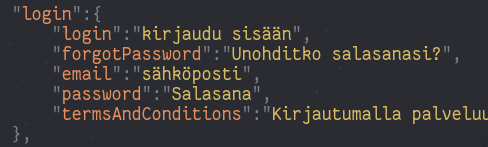
\includegraphics[width= 15cm, height=5cm]{src/public/jsonfixed.png} \\
\medskip
Kuva starttaamon suomenkielisen sisäänkirjautumissivun käännöksestä.
\medskip

Kuvassa näkyy sivun sisäänkirjautumissivun (engl. login) käyttämät suomenkieliset käännökset. Avain on englanniksi kirjoitettu merkkijono, jolla käyttöliittymä hakee käännökset. Arvo on merkkijono mikä ilmenee käyttöliittymälle.
Esimerkiksi saksankielisessä käännöstiedostossa arvo käännettäisi saksaksi.

\medskip

Kielen vaihtoon tarvitaan valikko, josta käyttäjä voi valita millä kielellä hän haluaa käyttää nettisivua. 
Tähän päätin rakentaa laskuvalikon, jossa eri kielet ovat kuvattuna lipuilla.
\medskip





\medskip

\includegraphics[width= 5cm, height=10cm]{src/public/locale_laskuvalikko.png} \\
\medskip
Kuva Laskuvalikosta.
\medskip

Kuvassa näkyy laskuvalikko, jossa kielet on esitetty lippuina.
Liput toimivat nopeina visuaalisina vihjeinä, jotka auttavat käyttäjiä tunnistamaan haluamansa kielen.
Kuvassa olevaan laskuvalikkoon voi lisätä kieliä helposti, mutta usean kielen lisääminen tuo ongelmia käyttöliittymän kanssa, koska laskuvalikko kasvaa ainoastaan alaspäin.
Jos sovellukseen pitäisi lisätä monta eri kieltä, laskuvalikon pitäisi pystyä kasvamaan myös sivusuunnassa ja siihen pitäisi lisätä hakemisto, millä käyttäjä voi hakea haluttua kieltä.
\medskip



\subsection*{Viikon Yhteenveto}


Viikkojen aikana opin käyttämään i18n kirjastoa ja ymmärsin miten käännökset ja lokalisointi toimii nettisivuilla.
Käännökset tämän kokoiseen projektiin on iso työ ja niiden toteuttamiseen kului useita viikkoja.
I18n kirjaston kanssa oli helppo tehdä työtä ja sen dokumentaatio oli kattava.
\medskip

Sovelluksella on nyt keskitetty paikka missä kaikki julkipuolen teksti on, ja koska käännökset on eritelty niille sivuille mihin ne kuuluvat on niiden etsiminen helppoa.
Keskitetty tekstipankki auttaa sovelluksen kehittämisessä tulevaisuudessa, sillä jos haluaa etsiä tekstiä sivuilta ei tarvitse alkaa etsimään komponentteja missä teksti sijaitsee, vaan etsiä se käännöstiedostosta.\medskip

Laskuvalikkoon kielien lisääminen on helppoa, mutta liian monen kielen lisääminen tekee valikosta vaikeakäyttöisen, sillä se kasvaa vain alaspäin.
Laskuvalikkoa voi jatkokehittää lisäämällä siihen ominaisuus, jolla käyttäjä voisi hakea kieliä ja kasvattaa valikkoa sivusuuntaisesti kun tarpeeksi monta kieltä on lisätty.
